\documentclass[a4paper,twoside]{article} 
\usepackage{texthanglist}
\usepackage{multicol}
\usepackage{changepage}
\usepackage{float}
\usepackage{grffile}
\usepackage{graphicx}
\usepackage{amssymb}
\usepackage{fontspec}
\usepackage{fancyhdr}
\usepackage{multicol}
\usepackage{calc}
\usepackage[margin=1cm,includeheadfoot]{geometry}
\usepackage{eso-pic}
\pagestyle{plain}\pagestyle{fancy}
\fancyhead{}
\fancyhead[LO]{\rightmark}
\fancyhead[RO]{\thepage}
\fancyhead[LE]{\thepage}
\fancyhead[RE]{\leftmark}
\renewcommand{\headrulewidth}{0.4pt} \renewcommand{\footrulewidth}{0.4pt}

\begin{document} 
\pagestyle{plain} 
\font\spanenentryletDatadicBody="Times New Roman" at 12pt
\font\spantexitemtespanentranslationsexamplessensesensesentryletDatadicBody="Gautami" at 10pt
\font\xitemtespanentranslationsexamplessensesensesentryletDatadicBody="Gautami" at 10pt
\font\spanenspanenspanentranslationsexamplessensesensesentryletDatadicBody="Times New Roman" at 12pt
\font\spanenspanentranslationsexamplessensesensesentryletDatadicBody="Times New Roman" at 12pt
\font\spanentranslationsexamplessensesensesentryletDatadicBody="Times New Roman" at 12pt
\font\spanenLexSensepublishStemGlossPubLesensesensesentryletDatadicBody="Times New Roman" at 10pt
\font\spanhiLexSensepublishStemGlossPubLesensesensesentryletDatadicBody="Arial Unicode MS" at 10pt
\font\LexSensepublishStemGlossPubLesensesensesentryletDatadicBody="Arial Unicode MS" at 10pt
\font\spanenspanenpictureCaptionpictureRightentryletDatadicBody="Times New Roman" at 12pt
\font\spanenpictureCaptionpictureRightentryletDatadicBody="Times New Roman" at 12pt
\font\spanenCmPicturepublishStemPileThumbnailPubpictureCaptionpictureRightentryletDatadicBody="Times New Roman" at 12pt
\font\CmPicturepublishStemPileThumbnailPubpictureCaptionpictureRightentryletDatadicBody="Times New Roman" at 12pt
\font\pictureCaptionpictureRightentryletDatadicBody="Times New Roman" at 12pt
\font\picturepictureRightentryletDatadicBody="Times New Roman" at 12pt
\font\pictureRightentryletDatadicBody="Times New Roman" at 12pt
\font\spanencomplexformrefsentryletDatadicBody="Times New Roman" at 12pt
\font\spanencomplexformformcomplexformrefsentryletDatadicBody="Times New Roman/B" at 10pt
\font\complexformformcomplexformrefsentryletDatadicBody="Gautami/B" at 10pt
\font\spanenspanencomplexformtypecomplexformrefsentryletDatadicBody="Times New Roman" at 12pt
\font\spanencomplexformtypecomplexformrefsentryletDatadicBody="Times New Roman" at 12pt
\font\complexformtypecomplexformrefsentryletDatadicBody="Times New Roman" at 12pt
\font\complexformrefsentryletDatadicBody="Times New Roman" at 12pt
\font\spanentranslationLdtranslationsexamplessensesensesentryletDatadicBody="Times New Roman" at 10pt
\font\spantetranslationLdtranslationsexamplessensesensesentryletDatadicBody="Gautami" at 10pt
\font\translationLdtranslationsexamplessensesensesentryletDatadicBody="Gautami" at 10pt
\font\translationsexamplessensesensesentryletDatadicBody="Times New Roman" at 12pt
\font\spanenexampleexamplessensesensesentryletDatadicBody="Times New Roman/I" at 10pt
\font\spanggoTeluINexampleexamplessensesensesentryletDatadicBody="Gautami/I" at 10pt
\font\exampleexamplessensesensesentryletDatadicBody="Gautami/I" at 10pt
\font\LexEntrypublishStemComponentTargetHeadWordRefaentryrefcomponentprimaryrefsentryletDatadicBody="Gautami/B" at 10pt
\font\aentryrefcomponentprimaryrefsentryletDatadicBody="Times New Roman" at 12pt
\font\entryrefcomponentprimaryrefsentryletDatadicBody="Times New Roman" at 12pt
\font\spanenspanenentryreftypeprimaryrefsentryletDatadicBody="Times New Roman" at 12pt
\font\spanenentryreftypeprimaryrefsentryletDatadicBody="Times New Roman" at 12pt
\font\entryreftypeprimaryrefsentryletDatadicBody="Times New Roman" at 12pt
\font\spanenprimaryrefsentryletDatadicBody="Times New Roman" at 12pt
\font\primaryrefsentryletDatadicBody="Times New Roman" at 12pt
\font\spanenexamplessensesensesentryletDatadicBody="Times New Roman" at 12pt
\font\spanentranslationLdtranslationsxitemexamplessensesensesentryletDatadicBody="Times New Roman" at 10pt
\font\spantetranslationLdtranslationsxitemexamplessensesensesentryletDatadicBody="Gautami" at 10pt
\font\translationLdtranslationsxitemexamplessensesensesentryletDatadicBody="Gautami" at 10pt
\font\translationsxitemexamplessensesensesentryletDatadicBody="Times New Roman" at 12pt
\font\spanenexamplexitemexamplessensesensesentryletDatadicBody="Times New Roman/I" at 10pt
\font\spanggoTeluINexamplexitemexamplessensesensesentryletDatadicBody="Gautami/I" at 10pt
\font\examplexitemexamplessensesensesentryletDatadicBody="Gautami/I" at 10pt
\font\xitemexamplessensesensesentryletDatadicBody="Times New Roman" at 12pt
\font\examplessensesensesentryletDatadicBody="Times New Roman" at 12pt
\font\spanhixitemhiLexSensepublishStemGlossPubLdsensesensesentryletDatadicBody="Arial Unicode MS" at 10pt
\font\xitemhiLexSensepublishStemGlossPubLdsensesensesentryletDatadicBody="Arial Unicode MS" at 10pt
\font\spantexitemteLexSensepublishStemGlossPubLdsensesensesentryletDatadicBody="Gautami" at 10pt
\font\xitemteLexSensepublishStemGlossPubLdsensesensesentryletDatadicBody="Gautami" at 10pt
\font\xsensenumberaftersensesensesentryletDatadicBody="Times New Roman" at 12pt
\font\xsensenumbersensesensesentryletDatadicBody="Times New Roman" at 12pt
\font\spanenspanengrammaticalinfoentryletDatadicBody="Times New Roman/I" at 10pt
\font\spanengrammaticalinfoentryletDatadicBody="Times New Roman/I" at 10pt
\font\grammaticalinfoentryletDatadicBody="Times New Roman/I" at 10pt
\font\spanensensesentryletDatadicBody="Times New Roman" at 12pt
\font\spanenLexSensepublishStemGlossPubLdsensesensesentryletDatadicBody="Times New Roman" at 10pt
\font\spanteLexSensepublishStemGlossPubLdsensesensesentryletDatadicBody="Gautami" at 10pt
\font\LexSensepublishStemGlossPubLdsensesensesentryletDatadicBody="Gautami" at 10pt
\font\spanenspanensensesensesentryletDatadicBody="Times New Roman" at 12pt
\font\spanensensesensesentryletDatadicBody="Times New Roman" at 12pt
\font\spanenspanengrammaticalinfosensesensesentryletDatadicBody="Times New Roman/I" at 10pt
\font\spanengrammaticalinfosensesensesentryletDatadicBody="Times New Roman/I" at 10pt
\font\grammaticalinfosensesensesentryletDatadicBody="Times New Roman/I" at 10pt
\font\sensesensesentryletDatadicBody="Times New Roman" at 12pt
\font\sensesentryletDatadicBody="Times New Roman" at 12pt
\font\spanenpronunciationsentryletDatadicBody="Times New Roman" at 12pt
\font\spanggofonipaxemicpronunciationpronunciationsentryletDatadicBody="Tahoma" at 10pt
\font\spanenpronunciationpronunciationsentryletDatadicBody="Times New Roman" at 10pt
\font\pronunciationpronunciationsentryletDatadicBody="Tahoma" at 10pt
\font\pronunciationsentryletDatadicBody="Times New Roman" at 12pt
\font\spanenheadwordentryletDatadicBody="Times New Roman/B" at 10pt
\font\headwordentryletDatadicBody="Gautami/B" at 10pt
\font\entryletDatadicBody="Times New Roman" at 12pt
\font\letDatadicBody="Times New Roman" at 12pt
\font\letterletHeaddicBody="Gautami/B" at 24pt
\font\letHeaddicBody="Times New Roman" at 12pt
\font\xitemtpi="Times New Roman" at 12pt
\font\xitemxitemtranslationLdbefore="Gautami" at 10pt
\font\xitemxitemtranslationbefore="Times New Roman" at 12pt
\font\sensesensesensesbefore="Times New Roman" at 12pt
\font\xitemxitempronunciationsbefore="Times New Roman" at 12pt
\font\xitemxitempronunciationbefore="Tahoma" at 10pt
\font\xitemxitemprimaryrefsbefore="Times New Roman" at 12pt
\font\xitemxitempictureLabelbefore="Times New Roman" at 12pt
\font\xitemxitempartofspeechbefore="Times New Roman" at 12pt
\font\xitemxitemLexSensepublishStemGlossPubLebefore="Arial Unicode MS" at 10pt
\font\xitemxitemLexSensepublishStemGlossPubLdbefore="Gautami" at 10pt
\font\xitemxitemLexEntryTypepublishStemEntryTypeAbbreviationPubbefore="Times New Roman" at 12pt
\font\xitemxitemLexEntryTypepublishStemComplexFormTypeReverseAbbrPubbefore="Times New Roman" at 12pt
\font\xitemxitemLexEntrypublishStemComponentTargetHeadWordRefbefore="Gautami/B" at 10pt
\font\xitemxitemheadwordbefore="Gautami/B" at 10pt
\font\xitemxitemexamplesbefore="Times New Roman" at 12pt
\font\xitemxitemexamplebefore="Gautami/I" at 10pt
\font\xitemxitementryreftypebefore="Times New Roman" at 12pt
\font\xitemxitementryrefcomponentbefore="Times New Roman" at 12pt
\font\xitemxitemdefinitionbefore="Times New Roman" at 12pt
\font\xitemxitemcomplexformrefsbefore="Times New Roman" at 12pt
\font\xitemxitemcomplexformformbefore="Gautami/B" at 10pt
\font\xitemhi="Arial Unicode MS" at 10pt
\font\xitemte="Gautami" at 10pt
\font\spanzhCN="SimSun" at 12pt
\font\divzhCN="SimSun" at 12pt
\font\spanur="Times New Roman" at 12pt
\font\divur="Times New Roman" at 12pt
\font\spanurxind="Times New Roman" at 12pt
\font\divurxind="Times New Roman" at 12pt
\font\spantr="Charis SIL" at 12pt
\font\divtr="Charis SIL" at 12pt
\font\spantrfonipa="Doulos SIL" at 12pt
\font\divtrfonipa="Doulos SIL" at 12pt
\font\spantrfonipaxemic="Times New Roman" at 12pt
\font\divtrfonipaxemic="Times New Roman" at 12pt
\font\spantpi="Times New Roman" at 12pt
\font\divtpi="Times New Roman" at 12pt
\font\spante="Gautami" at 12pt
\font\divte="Gautami" at 12pt
\font\spanseh="Doulos SIL" at 12pt
\font\divseh="Doulos SIL" at 12pt
\font\spanru="Times New Roman" at 12pt
\font\divru="Times New Roman" at 12pt
\font\spanqaaxcam="Times New Roman" at 12pt
\font\divqaaxcam="Times New Roman" at 12pt
\font\spanpt="Times New Roman" at 12pt
\font\divpt="Times New Roman" at 12pt
\font\spannko="Charis SIL" at 12pt
\font\divnko="Charis SIL" at 12pt
\font\spanmy="Padauk" at 12pt
\font\divmy="Padauk" at 12pt
\font\spanko="Gulim" at 12pt
\font\divko="Gulim" at 12pt
\font\spanid="Times New Roman" at 12pt
\font\divid="Times New Roman" at 12pt
\font\spanhi="Arial Unicode MS" at 12pt
\font\divhi="Arial Unicode MS" at 12pt
\font\spanhe="Ezra SIL" at 12pt
\font\divhe="Ezra SIL" at 12pt
\font\spanhbo="Ezra SIL" at 12pt
\font\divhbo="Ezra SIL" at 12pt
\font\spangrc="Galatia SIL" at 12pt
\font\divgrc="Galatia SIL" at 12pt
\font\spanggoTeluIN="Gautami" at 12pt
\font\divggoTeluIN="Gautami" at 12pt
\font\spanggofonipaxemic="Tahoma" at 12pt
\font\divggofonipaxemic="Tahoma" at 12pt
\font\spanfr="Times New Roman" at 12pt
\font\divfr="Times New Roman" at 12pt
\font\spanfa="Times New Roman" at 12pt
\font\divfa="Times New Roman" at 12pt
\font\spanes="Times New Roman" at 12pt
\font\dives="Times New Roman" at 12pt
\font\spanen="Times New Roman" at 12pt
\font\diven="Times New Roman" at 12pt
\font\spanenQaaaxtest="Charis SIL Compact" at 12pt
\font\divenQaaaxtest="Charis SIL Compact" at 12pt
\font\spanenfonipa="Doulos SIL" at 12pt
\font\divenfonipa="Doulos SIL" at 12pt
\font\spande="Times New Roman" at 12pt
\font\divde="Times New Roman" at 12pt
\font\spanbzh="Charis SIL" at 12pt
\font\divbzh="Charis SIL" at 12pt
\font\spanbzhfonipa="Doulos SIL" at 12pt
\font\divbzhfonipa="Doulos SIL" at 12pt
\font\spanbss="Charis SIL" at 12pt
\font\divbss="Charis SIL" at 12pt
\font\spanbssxako="Charis SIL Compact" at 12pt
\font\divbssxako="Charis SIL Compact" at 12pt
\font\spanbssfonipa="Charis SIL Compact" at 12pt
\font\divbssfonipa="Charis SIL Compact" at 12pt
\color{black} 
\AddToShipoutPicture*{% 
\put(0,0){\rule{\paperwidth}{\paperheight}}{
\includegraphics[width=\paperwidth, height=\paperheight]{cover.png}}% 
} 
\thispagestyle{empty} 
\font\CoverPageHeading="Times New Roman/B":color=000000 at 22pt 
\vskip 60pt 
\begin{center} 
\CoverPageHeading{Gondwana Sample} 
\end{center} 
\newpage 
\newpage 
\thispagestyle{empty} 
\mbox{} 

\pagestyle{fancy} 
\begin{center}
\topskip 18pt{\baselineskip 18pt{\letterletHeaddicBody{అ}}}
 \label{first_pageఅ} \end{center}
 \setlength{\columnsep}{12pt} 
\setlength\columnseprule{0.4pt} 
\begin{multicols}{2}{\raggedright} \begin{adjustwidth}{1pt}{0pt}{2pt}{9pt}
 \begin{hanglist}[12pt] \item 
\leftmargin 0pt{\markboth{ \headwordentryletDatadicBody అకుర్పొక్ (మహ్న)}{ \headwordentryletDatadicBody అకుర్పొక్ (మహ్న)}\headwordentryletDatadicBody{అకుర్పొక్ (మహ్న)}} \spanenpronunciationpronunciationsentryletDatadicBody{[}\spanggofonipaxemicpronunciationpronunciationsentryletDatadicBody{akurpok (mahna)}\spanenpronunciationpronunciationsentryletDatadicBody{]} \spanenspanengrammaticalinfosensesensesentryletDatadicBody{n} \spanenspanensensesensesentryletDatadicBody{month 6 of the Gond year (August-September).} \spanteLexSensepublishStemGlossPubLdsensesensesentryletDatadicBody{భాద్రపదం} \end{hanglist} \end{adjustwidth} 
\begin{adjustwidth}{1pt}{0pt}{2pt}{9pt}
 \begin{hanglist}[12pt] \item 
\leftmargin 0pt{\markboth{ \headwordentryletDatadicBody అకుర్పొక్ (మహ్న)}{ \headwordentryletDatadicBody అకుర్పొక్ (మహ్న)}\headwordentryletDatadicBody{అక్కల్}} \spanenpronunciationpronunciationsentryletDatadicBody{[}\spanggofonipaxemicpronunciationpronunciationsentryletDatadicBody{akkal}\spanenpronunciationpronunciationsentryletDatadicBody{]} \spanenspanengrammaticalinfoentryletDatadicBody{n} \xsensenumbersensesensesentryletDatadicBody{1}\xsensenumberaftersensesensesentryletDatadicBody{) }\spanteLexSensepublishStemGlossPubLdsensesensesentryletDatadicBody{బుద్ధి} \xsensenumbersensesensesentryletDatadicBody{2}\xsensenumberaftersensesensesentryletDatadicBody{) }\spanenspanensensesensesentryletDatadicBody{wisdom.} \spantexitemteLexSensepublishStemGlossPubLdsensesensesentryletDatadicBody{తెలివి} \spanhixitemhiLexSensepublishStemGlossPubLdsensesensesentryletDatadicBody{बुद्धि} \spanggoTeluINexamplexitemexamplessensesensesentryletDatadicBody{అక్కల్ మన్వల్ మాయ్నల్ చొకొట్ మందంతొర్.} \spantetranslationLdtranslationsxitemexamplessensesensesentryletDatadicBody{బుద్ధి గల వ్యక్తి మంచిగా ఉంటాడు.} \spanggoTeluINexamplexitemexamplessensesensesentryletDatadicBody{బయ్యె బాబలిర్ కాండిన్ అక్కల్ బుద్ది కరుసన.} \spantetranslationLdtranslationsxitemexamplessensesensesentryletDatadicBody{తండ్రి తల్లి కొడుకులను తెలివి తేటలు నేర్పాలి.} \end{hanglist} \end{adjustwidth} 
\begin{adjustwidth}{1pt}{0pt}{2pt}{9pt}
 \begin{hanglist}[12pt] \item 
\leftmargin 0pt{\markboth{ \headwordentryletDatadicBody అక్కల్}{ \headwordentryletDatadicBody అక్కల్}\headwordentryletDatadicBody{అక్కొ మామల}} \spanenpronunciationpronunciationsentryletDatadicBody{[}\spanggofonipaxemicpronunciationpronunciationsentryletDatadicBody{akko māmal}\spanenpronunciationpronunciationsentryletDatadicBody{]} \spanenprimaryrefsentryletDatadicBody{(}\spanenspanenentryreftypeprimaryrefsentryletDatadicBody{der. of} \leftmargin 0pt{\LexEntrypublishStemComponentTargetHeadWordRefaentryrefcomponentprimaryrefsentryletDatadicBody{అక్కొ మామల్}}\spanenprimaryrefsentryletDatadicBody{) }\spanenspanengrammaticalinfosensesensesentryletDatadicBody{n} \spanteLexSensepublishStemGlossPubLdsensesensesentryletDatadicBody{తాత మామయ్య} \spanggoTeluINexampleexamplessensesensesentryletDatadicBody{నన్ అక్కొ మామలిర్ సోరిక్ దాంతొన్.} \spantetranslationLdtranslationsexamplessensesensesentryletDatadicBody{నేనూ తాతయ్య మామయ్య ఇంటికి సంబంధానికి వెలుతాను.} \end{hanglist} \end{adjustwidth} 
\begin{adjustwidth}{1pt}{0pt}{2pt}{9pt}
 \begin{hanglist}[12pt] \item 
\leftmargin 0pt{\markboth{ \headwordentryletDatadicBody అక్కొ మామల}{ \headwordentryletDatadicBody అక్కొ మామల}\headwordentryletDatadicBody{అక్కొ మామల్}} \spanenpronunciationpronunciationsentryletDatadicBody{[}\spanggofonipaxemicpronunciationpronunciationsentryletDatadicBody{akko}\spanenpronunciationpronunciationsentryletDatadicBody{]} \spanenspanengrammaticalinfosensesensesentryletDatadicBody{n} \spanenspanensensesensesentryletDatadicBody{maternal grandfather.} \spantexitemteLexSensepublishStemGlossPubLdsensesensesentryletDatadicBody{తాత} \spanhixitemhiLexSensepublishStemGlossPubLdsensesensesentryletDatadicBody{तात; नानादादा; बूढा आदमी} \spanggoTeluINexamplexitemexamplessensesensesentryletDatadicBody{మావొర్ అక్కొ డగుర్.} \spantetranslationLdtranslationsxitemexamplessensesensesentryletDatadicBody{మా తాతయ్య పెద్దవాడు.} \spanggoTeluINexamplexitemexamplessensesensesentryletDatadicBody{అక్కొ చుట్ట ఉంజెర్ మంతొర్.} \spantetranslationLdtranslationsxitemexamplessensesensesentryletDatadicBody{తాతయ్య చుట్ట తాగుతున్నాడు.} \spanenspanencomplexformtypecomplexformrefsentryletDatadicBody{der.} \leftmargin 0pt{\complexformformcomplexformrefsentryletDatadicBody{అక్కొ మామల}} \end{hanglist} \end{adjustwidth} 
\begin{adjustwidth}{1pt}{0pt}{2pt}{9pt}
 \begin{hanglist}[12pt] \item 
\leftmargin 0pt{\markboth{ \headwordentryletDatadicBody అక్కొ మామల్}{ \headwordentryletDatadicBody అక్కొ మామల్}\headwordentryletDatadicBody{అక్డెమాత}} \spanenpronunciationpronunciationsentryletDatadicBody{[}\spanggofonipaxemicpronunciationpronunciationsentryletDatadicBody{akḍemāta}\spanenpronunciationpronunciationsentryletDatadicBody{]} \spanteLexSensepublishStemGlossPubLdsensesensesentryletDatadicBody{ముడ్చుకున్నది} \spanggoTeluINexampleexamplessensesensesentryletDatadicBody{నావంగ్ కాల్క్ అక్డెమాతంగ్.} \spantetranslationLdtranslationsexamplessensesensesentryletDatadicBody{నా కాళ్లు ముడ్చుకున్నాయి.} \end{hanglist} \end{adjustwidth} 
\begin{adjustwidth}{1pt}{0pt}{2pt}{9pt}
 \begin{hanglist}[12pt] \item 
\leftmargin 0pt{\markboth{ \headwordentryletDatadicBody అక్డెమాత}{ \headwordentryletDatadicBody అక్డెమాత}\headwordentryletDatadicBody{అక్ర}} \spanenpronunciationpronunciationsentryletDatadicBody{[}\spanggofonipaxemicpronunciationpronunciationsentryletDatadicBody{akra}\spanenpronunciationpronunciationsentryletDatadicBody{]} \spanenspanengrammaticalinfosensesensesentryletDatadicBody{num} \spanenspanensensesensesentryletDatadicBody{eleven.} \spantexitemteLexSensepublishStemGlossPubLdsensesensesentryletDatadicBody{(11) పదకొండు} \spanhixitemhiLexSensepublishStemGlossPubLdsensesensesentryletDatadicBody{ग्यारह} \spanggoTeluINexampleexamplessensesensesentryletDatadicBody{నాకున్ అక్ర హెర్రెంగ్ మంతంగ్.} \spantetranslationLdtranslationsexamplessensesensesentryletDatadicBody{నాకు పదకొండు మేకలు ఉన్నాయి.} \end{hanglist} \end{adjustwidth} 
\begin{adjustwidth}{1pt}{0pt}{2pt}{9pt}
 \begin{hanglist}[12pt] \item 
\leftmargin 0pt{\markboth{ \headwordentryletDatadicBody అక్ర}{ \headwordentryletDatadicBody అక్ర}\headwordentryletDatadicBody{అక్సర్}} \spanenpronunciationpronunciationsentryletDatadicBody{[}\spanggofonipaxemicpronunciationpronunciationsentryletDatadicBody{aksar}\spanenpronunciationpronunciationsentryletDatadicBody{]} \spanenspanengrammaticalinfosensesensesentryletDatadicBody{n} \spanenspanensensesensesentryletDatadicBody{characters} \spanteLexSensepublishStemGlossPubLdsensesensesentryletDatadicBody{అక్షరాలు} \spanggoTeluINexampleexamplessensesensesentryletDatadicBody{మస్తరల్ అక్సర్కున్ వెహ్తొర్.} \spantetranslationLdtranslationsexamplessensesensesentryletDatadicBody{గురువు అక్షరాలు చెప్పాడు.} \end{hanglist} \end{adjustwidth} 
\begin{adjustwidth}{1pt}{0pt}{2pt}{9pt}
 \begin{hanglist}[12pt] \item 
\leftmargin 0pt{\markboth{ \headwordentryletDatadicBody అక్సర్}{ \headwordentryletDatadicBody అక్సర్}\headwordentryletDatadicBody{అక్సర్క్‌నె}} \spanenpronunciationpronunciationsentryletDatadicBody{[}\spanggofonipaxemicpronunciationpronunciationsentryletDatadicBody{aksarkne}\spanenpronunciationpronunciationsentryletDatadicBody{]} \spanteLexSensepublishStemGlossPubLdsensesensesentryletDatadicBody{అచ్చరాలతో} \spanggoTeluINexampleexamplessensesensesentryletDatadicBody{గోండి బాసతున్ అక్సర్క్‌నె లిహి కీంతెర్.} \spantetranslationLdtranslationsexamplessensesensesentryletDatadicBody{గోండిని అచ్చరాలలో రాసుకుంటారు.} \end{hanglist} \end{adjustwidth} 
\begin{adjustwidth}{1pt}{0pt}{2pt}{9pt}
 \begin{hanglist}[12pt] \item \begin{adjustwidth}{2pt}{2pt}{2pt}{2pt}\begin{center}

\begin{wrapfigure}
\begin{center}
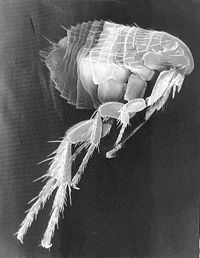
\includegraphics[angle=0,width=54mm,height=36mm]{1.jpg} 
\caption{}
\end{center}
\end{wrapfigure}



\spanenspanenpictureCaptionpictureRightentryletDatadicBody{rice with tumeric}
\end{center}\end{adjustwidth}  
\leftmargin 0pt{\markboth{ \headwordentryletDatadicBody అక్సర్క్‌నె}{ \headwordentryletDatadicBody అక్సర్క్‌నె}\headwordentryletDatadicBody{అక్సెదంగ్}} \spanenpronunciationpronunciationsentryletDatadicBody{[}\spanggofonipaxemicpronunciationpronunciationsentryletDatadicBody{aksedaṅg}\spanenpronunciationpronunciationsentryletDatadicBody{]} \spanenspanengrammaticalinfoentryletDatadicBody{n} \xsensenumbersensesensesentryletDatadicBody{1}\xsensenumberaftersensesensesentryletDatadicBody{) }\spanenspanensensesensesentryletDatadicBody{rice with vermilion} \spanteLexSensepublishStemGlossPubLdsensesensesentryletDatadicBody{పసుపు బియ్యం} \xsensenumbersensesensesentryletDatadicBody{2}\xsensenumberaftersensesensesentryletDatadicBody{) }\spanenspanensensesensesentryletDatadicBody{rice mixed with vermilion thrown at a wedding, or on cattle (e.g. during 'laxmi pooja') in order to bless.} \spanhiLexSensepublishStemGlossPubLesensesensesentryletDatadicBody{अक्षतब.; हल्दी और कुंकुम से मिश्रित चावल} \spanggoTeluINexampleexamplessensesensesentryletDatadicBody{గొవుర్ దన్ గోటమ్నె నొవ్రి నొవ్రనగ సమ్దిర్ అక్సెదాంగ్ వాటంతెర్.} \spanenspanenspanentranslationsexamplessensesensesentryletDatadicBody{At the wedding place, everyone throws rice on the bride andgroom.} \spantexitemtespanentranslationsexamplessensesensesentryletDatadicBody{$\sharp$పెండ్లి పందిరిలో పడుసు, వరులకు పసుపు బియ్యం వేస్తారు.} \end{hanglist} \end{adjustwidth} 
\begin{adjustwidth}{1pt}{0pt}{2pt}{9pt}
 \begin{hanglist}[12pt] \item 
\leftmargin 0pt{\markboth{ \headwordentryletDatadicBody అక్సెదంగ్}{ \headwordentryletDatadicBody అక్సెదంగ్}\headwordentryletDatadicBody{అక్సెదన దివొస్}} \spanenpronunciationpronunciationsentryletDatadicBody{[}\spanggofonipaxemicpronunciationpronunciationsentryletDatadicBody{aksedana divos}\spanenpronunciationpronunciationsentryletDatadicBody{]} \spanenspanensensesensesentryletDatadicBody{wedding day} \spanteLexSensepublishStemGlossPubLdsensesensesentryletDatadicBody{పెళ్లి రోజు} \end{hanglist} \end{adjustwidth} 
\begin{adjustwidth}{1pt}{0pt}{2pt}{9pt}
 \begin{hanglist}[12pt] \item 
\leftmargin 0pt{\markboth{ \headwordentryletDatadicBody అక్సెదన దివొస్}{ \headwordentryletDatadicBody అక్సెదన దివొస్}\headwordentryletDatadicBody{అక్సెర్}} \spanenpronunciationpronunciationsentryletDatadicBody{[}\spanggofonipaxemicpronunciationpronunciationsentryletDatadicBody{akser}\spanenpronunciationpronunciationsentryletDatadicBody{]} \spanenspanengrammaticalinfosensesensesentryletDatadicBody{n} \spanenspanensensesensesentryletDatadicBody{character} \spantexitemteLexSensepublishStemGlossPubLdsensesensesentryletDatadicBody{అక్షరం} \spanhixitemhiLexSensepublishStemGlossPubLdsensesensesentryletDatadicBody{अक्षर; वर्ण} \spanggoTeluINexampleexamplessensesensesentryletDatadicBody{అక్సెర్ ఉంది గునం.} \spantetranslationLdtranslationsexamplessensesensesentryletDatadicBody{అక్షరం ఉంది గుణం.} \end{hanglist} \end{adjustwidth} 
\begin{adjustwidth}{1pt}{0pt}{2pt}{9pt}
 \begin{hanglist}[12pt] \item 
\leftmargin 0pt{\markboth{ \headwordentryletDatadicBody అక్సెర్}{ \headwordentryletDatadicBody అక్సెర్}\headwordentryletDatadicBody{అగ్గటల్}} \spanenpronunciationpronunciationsentryletDatadicBody{[}\spanggofonipaxemicpronunciationpronunciationsentryletDatadicBody{aggaṭal}\spanenpronunciationpronunciationsentryletDatadicBody{]} \spanenspanengrammaticalinfoentryletDatadicBody{adv} \xsensenumbersensesensesentryletDatadicBody{1}\xsensenumberaftersensesensesentryletDatadicBody{) }\spanenspanensensesensesentryletDatadicBody{from there (nm.)} \spantexitemteLexSensepublishStemGlossPubLdsensesensesentryletDatadicBody{నుంచి} \spanhixitemhiLexSensepublishStemGlossPubLdsensesensesentryletDatadicBody{वहा से} \xsensenumbersensesensesentryletDatadicBody{2}\xsensenumberaftersensesensesentryletDatadicBody{) }\spanenspanensensesensesentryletDatadicBody{someone (nm.) or something from there.} \spanteLexSensepublishStemGlossPubLdsensesensesentryletDatadicBody{అక్కడనుండి} \spanggoTeluINexampleexamplessensesensesentryletDatadicBody{అగ్గటల్ నన్న నీకున్ సూడ్తొన్.} \spantetranslationLdtranslationsexamplessensesensesentryletDatadicBody{అక్కడి నుండి నేను నిన్ను చూసాను.} \end{hanglist} \end{adjustwidth} 
\begin{adjustwidth}{1pt}{0pt}{2pt}{9pt}
 \begin{hanglist}[12pt] \item 
\leftmargin 0pt{\markboth{ \headwordentryletDatadicBody అగ్గటల్}{ \headwordentryletDatadicBody అగ్గటల్}\headwordentryletDatadicBody{అగ్గటొర}} \spanenpronunciationpronunciationsentryletDatadicBody{[}\spanggofonipaxemicpronunciationpronunciationsentryletDatadicBody{aggaṭor}\spanenpronunciationpronunciationsentryletDatadicBody{]} \spanenprimaryrefsentryletDatadicBody{(}\spanenspanenentryreftypeprimaryrefsentryletDatadicBody{der. of} \leftmargin 0pt{\LexEntrypublishStemComponentTargetHeadWordRefaentryrefcomponentprimaryrefsentryletDatadicBody{అగ్గటొర్}}\spanenprimaryrefsentryletDatadicBody{) }\spanenspanengrammaticalinfosensesensesentryletDatadicBody{n} \spanenspanensensesensesentryletDatadicBody{man from there.} \spanteLexSensepublishStemGlossPubLdsensesensesentryletDatadicBody{అక్కడివారు} \spanggoTeluINexampleexamplessensesensesentryletDatadicBody{వేర్ మాయ్నల్ అగ్గటొర్.} \spanenspanenspanentranslationsexamplessensesensesentryletDatadicBody{This man is from there.} \spantexitemtespanentranslationsexamplessensesensesentryletDatadicBody{ఈ వ్యక్తి అక్కడి వారు.} \end{hanglist} \end{adjustwidth} 
\begin{adjustwidth}{1pt}{0pt}{2pt}{9pt}
 \begin{hanglist}[12pt] \item 
\leftmargin 0pt{\markboth{ \headwordentryletDatadicBody అగ్గటొర}{ \headwordentryletDatadicBody అగ్గటొర}\headwordentryletDatadicBody{అగ్గటొర్}} \spanenpronunciationpronunciationsentryletDatadicBody{[}\spanggofonipaxemicpronunciationpronunciationsentryletDatadicBody{agga}\spanenpronunciationpronunciationsentryletDatadicBody{]} \xsensenumbersensesensesentryletDatadicBody{1}\xsensenumberaftersensesensesentryletDatadicBody{) }\spanenspanengrammaticalinfosensesensesentryletDatadicBody{adv} \spanenspanensensesensesentryletDatadicBody{there.} \spantexitemteLexSensepublishStemGlossPubLdsensesensesentryletDatadicBody{అక్కడ} \spanhixitemhiLexSensepublishStemGlossPubLdsensesensesentryletDatadicBody{वहा} \spanggoTeluINexampleexamplessensesensesentryletDatadicBody{వేర్ వెర్తల్ అగ్గటొర్ ఆందుర్.} \spantetranslationLdtranslationsexamplessensesensesentryletDatadicBody{ఈ చుట్టము అక్కడి వాడు.} \xsensenumbersensesensesentryletDatadicBody{2}\xsensenumberaftersensesensesentryletDatadicBody{) }\spanenspanensensesensesentryletDatadicBody{there} \spanenspanencomplexformtypecomplexformrefsentryletDatadicBody{der.} \leftmargin 0pt{\complexformformcomplexformrefsentryletDatadicBody{అగ్గటొర}} \end{hanglist} \end{adjustwidth} 
\begin{adjustwidth}{1pt}{0pt}{2pt}{9pt}
 \begin{hanglist}[12pt] \item 
\leftmargin 0pt{\markboth{ \headwordentryletDatadicBody అగ్గటొర్}{ \headwordentryletDatadicBody అగ్గటొర్}\headwordentryletDatadicBody{అఙె}} \spanenpronunciationpronunciationsentryletDatadicBody{[}\spanggofonipaxemicpronunciationpronunciationsentryletDatadicBody{aṅe}\spanenpronunciationpronunciationsentryletDatadicBody{]} \spanenspanengrammaticalinfosensesensesentryletDatadicBody{n} \spanenspanensensesensesentryletDatadicBody{elder brother's wife.} \spantexitemteLexSensepublishStemGlossPubLdsensesensesentryletDatadicBody{వదిన} \spanhixitemhiLexSensepublishStemGlossPubLdsensesensesentryletDatadicBody{भाबि} \spanggoTeluINexampleexamplessensesensesentryletDatadicBody{మావొర్ దాదన బాయ్కొ నాకున్ అఙె ఆంత.} \spantetranslationLdtranslationsexamplessensesensesentryletDatadicBody{మా అన్నయ్య పెండ్లం నాకు వదిన అవుతుంది.} \end{hanglist} \end{adjustwidth} 
\begin{adjustwidth}{1pt}{0pt}{2pt}{9pt}
 \begin{hanglist}[12pt] \item 
\leftmargin 0pt{\markboth{ \headwordentryletDatadicBody అఙె}{ \headwordentryletDatadicBody అఙె}\headwordentryletDatadicBody{అచనక్}} \spanenpronunciationpronunciationsentryletDatadicBody{[}\spanggofonipaxemicpronunciationpronunciationsentryletDatadicBody{acanak}\spanenpronunciationpronunciationsentryletDatadicBody{]} \spanenspanengrammaticalinfosensesensesentryletDatadicBody{adv} \spanenspanensensesensesentryletDatadicBody{suddenly} \spanteLexSensepublishStemGlossPubLdsensesensesentryletDatadicBody{ఆకస్మికంగా} \spanggoTeluINexampleexamplessensesensesentryletDatadicBody{మావ సాడతె అచనక్ పి.ఓ. సాబ్ వాసి మత్తొర్.} \spantetranslationLdtranslationsexamplessensesensesentryletDatadicBody{మా బడికి పి.ఓ ఆకస్మికంగా వచ్చినాడు.} \end{hanglist} \end{adjustwidth} 
\begin{adjustwidth}{1pt}{0pt}{2pt}{9pt}
 \begin{hanglist}[12pt] \item 
\leftmargin 0pt{\markboth{ \headwordentryletDatadicBody అచనక్}{ \headwordentryletDatadicBody అచనక్}\headwordentryletDatadicBody{అచొట్క్}} \spanenpronunciationpronunciationsentryletDatadicBody{[}\spanggofonipaxemicpronunciationpronunciationsentryletDatadicBody{acoṭk}\spanenpronunciationpronunciationsentryletDatadicBody{]} \spanenspanengrammaticalinfosensesensesentryletDatadicBody{n} \spanenspanensensesensesentryletDatadicBody{usual} \spantexitemteLexSensepublishStemGlossPubLdsensesensesentryletDatadicBody{మామూలు} \spanhixitemhiLexSensepublishStemGlossPubLdsensesensesentryletDatadicBody{साधारण} \end{hanglist} \end{adjustwidth} 
\begin{adjustwidth}{1pt}{0pt}{2pt}{9pt}
 \begin{hanglist}[12pt] \item 
\leftmargin 0pt{\markboth{ \headwordentryletDatadicBody అచొట్క్}{ \headwordentryletDatadicBody అచొట్క్}\headwordentryletDatadicBody{అచ్చొరె}} \spanenpronunciationpronunciationsentryletDatadicBody{[}\spanggofonipaxemicpronunciationpronunciationsentryletDatadicBody{accore}\spanenpronunciationpronunciationsentryletDatadicBody{]} \xsensenumbersensesensesentryletDatadicBody{1}\xsensenumberaftersensesensesentryletDatadicBody{) }\spanteLexSensepublishStemGlossPubLdsensesensesentryletDatadicBody{ఇంతే} \spanggoTeluINexampleexamplessensesensesentryletDatadicBody{కాండిరంగ్ పరిక్సంగ్ అచ్చొరె.} \spantetranslationLdtranslationsexamplessensesensesentryletDatadicBody{పిల్లల పరీక్షలు ఇంతే.} \xsensenumbersensesensesentryletDatadicBody{2}\xsensenumberaftersensesensesentryletDatadicBody{) }\spanenspanensensesensesentryletDatadicBody{that's all} \end{hanglist} \end{adjustwidth} 
\begin{adjustwidth}{1pt}{0pt}{2pt}{9pt}
 \begin{hanglist}[12pt] \item 
\leftmargin 0pt{\markboth{ \headwordentryletDatadicBody అచ్చొరె}{ \headwordentryletDatadicBody అచ్చొరె}\headwordentryletDatadicBody{అచ్చొర్}} \spanenpronunciationpronunciationsentryletDatadicBody{[}\spanggofonipaxemicpronunciationpronunciationsentryletDatadicBody{accor}\spanenpronunciationpronunciationsentryletDatadicBody{]} \spanenspanengrammaticalinfosensesensesentryletDatadicBody{adv} \spanenspanensensesensesentryletDatadicBody{that much, that many (nm.).} \spanteLexSensepublishStemGlossPubLdsensesensesentryletDatadicBody{అంత} \spanggoTeluINexampleexamplessensesensesentryletDatadicBody{నిమ్మె అచ్చొర్ డగుర్ బహన్ ఆతి.} \spantetranslationLdtranslationsexamplessensesensesentryletDatadicBody{నీవు అంత పెద్దగా ఏలా అయినావు.} \spanenspanencomplexformtypecomplexformrefsentryletDatadicBody{der.} \leftmargin 0pt{\complexformformcomplexformrefsentryletDatadicBody{అచ్చోడ్ రొప్పొ}} \end{hanglist} \end{adjustwidth} 
\begin{adjustwidth}{1pt}{0pt}{2pt}{9pt}
 \begin{hanglist}[12pt] \item 
\leftmargin 0pt{\markboth{ \headwordentryletDatadicBody అచ్చొర్}{ \headwordentryletDatadicBody అచ్చొర్}\headwordentryletDatadicBody{అచ్చోడ్ రొప్పొ}} \spanenpronunciationpronunciationsentryletDatadicBody{[}\spanggofonipaxemicpronunciationpronunciationsentryletDatadicBody{accōḍ roppo}\spanenpronunciationpronunciationsentryletDatadicBody{]} \spanenprimaryrefsentryletDatadicBody{(}\spanenspanenentryreftypeprimaryrefsentryletDatadicBody{der. of} \leftmargin 0pt{\LexEntrypublishStemComponentTargetHeadWordRefaentryrefcomponentprimaryrefsentryletDatadicBody{అచ్చొర్}}\spanenprimaryrefsentryletDatadicBody{) }\spanenspanengrammaticalinfosensesensesentryletDatadicBody{adv} \spanenspanensensesensesentryletDatadicBody{meanwhile.} \spantexitemteLexSensepublishStemGlossPubLdsensesensesentryletDatadicBody{అంతలో} \spanhixitemhiLexSensepublishStemGlossPubLdsensesensesentryletDatadicBody{इसी दौरान} \spanggoTeluINexampleexamplessensesensesentryletDatadicBody{బుయరితగ అచ్చొడ్ రొప్పొ నేంగ్మా.} \spantetranslationLdtranslationsexamplessensesensesentryletDatadicBody{గుహలో చాల లోపలికి వెళ్లకు.} \end{hanglist} \end{adjustwidth} 
\begin{adjustwidth}{1pt}{0pt}{2pt}{9pt}
 \begin{hanglist}[12pt] \item 
\leftmargin 0pt{\markboth{ \headwordentryletDatadicBody అచ్చోడ్ రొప్పొ}{ \headwordentryletDatadicBody అచ్చోడ్ రొప్పొ}\headwordentryletDatadicBody{అచ్వీర్}} \spanenpronunciationpronunciationsentryletDatadicBody{[}\spanggofonipaxemicpronunciationpronunciationsentryletDatadicBody{acvīr}\spanenpronunciationpronunciationsentryletDatadicBody{]} \spanenspanengrammaticalinfosensesensesentryletDatadicBody{pro} \spanenspanensensesensesentryletDatadicBody{that many (m.).} \spanteLexSensepublishStemGlossPubLdsensesensesentryletDatadicBody{అంతమంది} \spanggoTeluINexampleexamplessensesensesentryletDatadicBody{అచ్విర్ తె మావ రోన్ తిన్లెన్ వాయన.} \spantetranslationLdtranslationsexamplessensesensesentryletDatadicBody{అంతమంది మా ఇంటికి తినడానికి రావాలి.} \end{hanglist} \end{adjustwidth} 
\begin{adjustwidth}{1pt}{0pt}{2pt}{9pt}
 \begin{hanglist}[12pt] \item 
\leftmargin 0pt{\markboth{ \headwordentryletDatadicBody అచ్వీర్}{ \headwordentryletDatadicBody అచ్వీర్}\headwordentryletDatadicBody{అజుక్}} \spanenpronunciationpronunciationsentryletDatadicBody{[}\spanggofonipaxemicpronunciationpronunciationsentryletDatadicBody{ajuk}\spanenpronunciationpronunciationsentryletDatadicBody{]} \spanenspanengrammaticalinfosensesensesentryletDatadicBody{conj} \spanenspanensensesensesentryletDatadicBody{even now.} \spanteLexSensepublishStemGlossPubLdsensesensesentryletDatadicBody{ఇంకా} \spanggoTeluINexampleexamplessensesensesentryletDatadicBody{దుకాన్ దారల్ అజుక్ ఉండె బతంగ్ పహజ్లె ఇంతొర్.} \spantetranslationLdtranslationsexamplessensesensesentryletDatadicBody{దుకాణ దారు ఇంకా ఏమి కావాలి అని అడుగుతున్నాడు.} \end{hanglist} \end{adjustwidth} 
\begin{adjustwidth}{1pt}{0pt}{2pt}{9pt}
 \begin{hanglist}[12pt] \item 
\leftmargin 0pt{\markboth{ \headwordentryletDatadicBody అజుక్}{ \headwordentryletDatadicBody అజుక్}\headwordentryletDatadicBody{అటుమ్ కుటుమ్}} \spanenpronunciationpronunciationsentryletDatadicBody{[}\spanggofonipaxemicpronunciationpronunciationsentryletDatadicBody{aṭum kuṭum}\spanenpronunciationpronunciationsentryletDatadicBody{]} \spanteLexSensepublishStemGlossPubLdsensesensesentryletDatadicBody{చుట్టలు చుట్టం} \spanggoTeluINexampleexamplessensesensesentryletDatadicBody{మర్మిన్క్ అటుమ్ కుటుమున్ సమ్దిర్క్ కేయంతెర్.} \spantetranslationLdtranslationsexamplessensesensesentryletDatadicBody{పెండ్లిలో చుట్టలు చుట్టాలు అందరిని పిలుస్తారు.} \end{hanglist} \end{adjustwidth} 
\begin{adjustwidth}{1pt}{0pt}{2pt}{9pt}
 \begin{hanglist}[12pt] \item 
\leftmargin 0pt{\markboth{ \headwordentryletDatadicBody అటుమ్ కుటుమ్}{ \headwordentryletDatadicBody అటుమ్ కుటుమ్}\headwordentryletDatadicBody{అటొ}} \spanenpronunciationpronunciationsentryletDatadicBody{[}\spanggofonipaxemicpronunciationpronunciationsentryletDatadicBody{aṭo}\spanenpronunciationpronunciationsentryletDatadicBody{]} \spanenspanengrammaticalinfosensesensesentryletDatadicBody{n} \spanenspanensensesensesentryletDatadicBody{auto} \spanteLexSensepublishStemGlossPubLdsensesensesentryletDatadicBody{ఆటో} \spanggoTeluINexampleexamplessensesensesentryletDatadicBody{అటొతున్ మూంద్ గారెంగ్ మందంతంగ్.} \spantetranslationLdtranslationsexamplessensesensesentryletDatadicBody{ఆటో కు మూడు చక్రాలు ఉంటాయి.} \end{hanglist} \end{adjustwidth} 
\begin{adjustwidth}{1pt}{0pt}{2pt}{9pt}
 \begin{hanglist}[12pt] \item 
\leftmargin 0pt{\markboth{ \headwordentryletDatadicBody అటొ}{ \headwordentryletDatadicBody అటొ}\headwordentryletDatadicBody{అట్కీ కీత}} \spanenpronunciationpronunciationsentryletDatadicBody{[}\spanggofonipaxemicpronunciationpronunciationsentryletDatadicBody{aṭki kī-}\spanenpronunciationpronunciationsentryletDatadicBody{]} \spanenspanengrammaticalinfoentryletDatadicBody{n} \xsensenumbersensesensesentryletDatadicBody{1}\xsensenumberaftersensesensesentryletDatadicBody{) }\spanenspanensensesensesentryletDatadicBody{fixation} \spanteLexSensepublishStemGlossPubLdsensesensesentryletDatadicBody{అంటించడం} \xsensenumbersensesensesentryletDatadicBody{2}\xsensenumberaftersensesensesentryletDatadicBody{) }\spanenspanensensesensesentryletDatadicBody{to hang.} \spanhiLexSensepublishStemGlossPubLesensesensesentryletDatadicBody{टाँगना} \spanggoTeluINexampleexamplessensesensesentryletDatadicBody{నావ ఆంగ్డెతున్ మోలతగ అట్కి కీతొన్.} \spantetranslationLdtranslationsexamplessensesensesentryletDatadicBody{నా అంగిని మొలలో అంటి పెట్టుకున్నాను.} \end{hanglist} \end{adjustwidth} 
\begin{adjustwidth}{1pt}{0pt}{2pt}{9pt}
 \begin{hanglist}[12pt] \item 
\leftmargin 0pt{\markboth{ \headwordentryletDatadicBody అట్కీ కీత}{ \headwordentryletDatadicBody అట్కీ కీత}\headwordentryletDatadicBody{అట్కుల్క్}} \spanenpronunciationpronunciationsentryletDatadicBody{[}\spanggofonipaxemicpronunciationpronunciationsentryletDatadicBody{aṭkulk}\spanenpronunciationpronunciationsentryletDatadicBody{]} \spanenspanengrammaticalinfosensesensesentryletDatadicBody{n} \spanenspanensensesensesentryletDatadicBody{flattened rice} \spantexitemteLexSensepublishStemGlossPubLdsensesensesentryletDatadicBody{అటుకులు} \spanhixitemhiLexSensepublishStemGlossPubLdsensesensesentryletDatadicBody{चिउडा} \spanggoTeluINexampleexamplessensesensesentryletDatadicBody{పెరెక్ ఙల్ అట్కుల్క్ తయర్ కీంతెర్.} \spantetranslationLdtranslationsexamplessensesensesentryletDatadicBody{బియ్యము నుండి అటుకులు తయారు చేస్తారు.} \end{hanglist} \end{adjustwidth} 
\begin{adjustwidth}{1pt}{0pt}{2pt}{9pt}
 \begin{hanglist}[12pt] \item 
\leftmargin 0pt{\markboth{ \headwordentryletDatadicBody అట్కుల్క్}{ \headwordentryletDatadicBody అట్కుల్క్}\headwordentryletDatadicBody{అట్కె మాత}} \spanenpronunciationpronunciationsentryletDatadicBody{[}\spanggofonipaxemicpronunciationpronunciationsentryletDatadicBody{aṭke māta}\spanenpronunciationpronunciationsentryletDatadicBody{]} \spanteLexSensepublishStemGlossPubLdsensesensesentryletDatadicBody{ఊపిరి ఆగింది} \spanggoTeluINexampleexamplessensesensesentryletDatadicBody{నావ నేస్క్‌వల్ అట్కె మాత.} \spantetranslationLdtranslationsexamplessensesensesentryletDatadicBody{నా ఊపిరి ఆగిపోయింది.} \end{hanglist} \end{adjustwidth} 
\begin{adjustwidth}{1pt}{0pt}{2pt}{9pt}
 \begin{hanglist}[12pt] \item 
\leftmargin 0pt{\markboth{ \headwordentryletDatadicBody అట్కె మాత}{ \headwordentryletDatadicBody అట్కె మాత}\headwordentryletDatadicBody{అట్ట}} \spanenpronunciationpronunciationsentryletDatadicBody{[}\spanggofonipaxemicpronunciationpronunciationsentryletDatadicBody{aṭṭa}\spanenpronunciationpronunciationsentryletDatadicBody{]} \spanenspanensensesensesentryletDatadicBody{cook} \spanteLexSensepublishStemGlossPubLdsensesensesentryletDatadicBody{వంట చెయ్యి} \end{hanglist} \end{adjustwidth} 
\begin{adjustwidth}{1pt}{0pt}{2pt}{9pt}
 \begin{hanglist}[12pt] \item 
\leftmargin 0pt{\markboth{ \headwordentryletDatadicBody అట్ట}{ \headwordentryletDatadicBody అట్ట}\headwordentryletDatadicBody{అట్టవన్}} \spanenpronunciationpronunciationsentryletDatadicBody{[}\spanggofonipaxemicpronunciationpronunciationsentryletDatadicBody{aṭṭavan}\spanenpronunciationpronunciationsentryletDatadicBody{]} \spanenspanengrammaticalinfosensesensesentryletDatadicBody{num} \spanenspanensensesensesentryletDatadicBody{fifty-eight.} \spantexitemteLexSensepublishStemGlossPubLdsensesensesentryletDatadicBody{(58) యాభై ఎనిమిది} \spanhixitemhiLexSensepublishStemGlossPubLdsensesensesentryletDatadicBody{अट्‌ठावन} \spanggoTeluINexampleexamplessensesensesentryletDatadicBody{మా కాండిన్ అట్టవన్ జోకఙ్ లిహికియుస్తోన్.} \spantetranslationLdtranslationsexamplessensesensesentryletDatadicBody{మా పిల్ల వానికి 50 ఎనిమిది సార్లు రాయించాను.} \end{hanglist} \end{adjustwidth} 
\begin{adjustwidth}{1pt}{0pt}{2pt}{9pt}
 \begin{hanglist}[12pt] \item 
\leftmargin 0pt{\markboth{ \headwordentryletDatadicBody అట్టవన్}{ \headwordentryletDatadicBody అట్టవన్}\headwordentryletDatadicBody{అట్టవీస్}} \spanenpronunciationpronunciationsentryletDatadicBody{[}\spanggofonipaxemicpronunciationpronunciationsentryletDatadicBody{aṭṭavīs}\spanenpronunciationpronunciationsentryletDatadicBody{]} \spanenspanengrammaticalinfosensesensesentryletDatadicBody{num} \spanenspanensensesensesentryletDatadicBody{twenty-eight.} \spantexitemteLexSensepublishStemGlossPubLdsensesensesentryletDatadicBody{(28) ఇరవై ఎనిమిది} \spanhixitemhiLexSensepublishStemGlossPubLdsensesensesentryletDatadicBody{अट्‌ठाईस} \spanggoTeluINexampleexamplessensesensesentryletDatadicBody{నన్ అట్టావీస్ న పొంటిన్ మా సాడకండిర్ కున్ యేత్‌తొన్.} \spantetranslationLdtranslationsexamplessensesensesentryletDatadicBody{మా బడి పిల్లలకు ఇరవై ఎనిమిది రూపాయిల పెన్నులు కొన్నాను.} \end{hanglist} \end{adjustwidth} 
\begin{adjustwidth}{1pt}{0pt}{2pt}{9pt}
 \begin{hanglist}[12pt] \item 
\leftmargin 0pt{\markboth{ \headwordentryletDatadicBody అట్టవీస్}{ \headwordentryletDatadicBody అట్టవీస్}\headwordentryletDatadicBody{అట్టెచాలిస్}} \spanenpronunciationpronunciationsentryletDatadicBody{[}\spanggofonipaxemicpronunciationpronunciationsentryletDatadicBody{aṭṭecālis}\spanenpronunciationpronunciationsentryletDatadicBody{]} \spanenspanengrammaticalinfosensesensesentryletDatadicBody{num} \spanenspanensensesensesentryletDatadicBody{forty-eight.} \spantexitemteLexSensepublishStemGlossPubLdsensesensesentryletDatadicBody{(48) నలభై ఎనిమిది} \spanhixitemhiLexSensepublishStemGlossPubLdsensesensesentryletDatadicBody{अड़तालीस} \spanggoTeluINexampleexamplessensesensesentryletDatadicBody{అద్ ఆంగ్డె అట్టె చాలిస్న ఆంద్.} \spantetranslationLdtranslationsexamplessensesensesentryletDatadicBody{ఆ చొక్క నలభై ఎనిమిది రూపాయలు.} \end{hanglist} \end{adjustwidth} 
\begin{adjustwidth}{1pt}{0pt}{2pt}{9pt}
 \begin{hanglist}[12pt] \item 
\leftmargin 0pt{\markboth{ \headwordentryletDatadicBody అట్టెచాలిస్}{ \headwordentryletDatadicBody అట్టెచాలిస్}\headwordentryletDatadicBody{అట్టెసాట్}} \spanenpronunciationpronunciationsentryletDatadicBody{[}\spanggofonipaxemicpronunciationpronunciationsentryletDatadicBody{aṭṭesāṭ}\spanenpronunciationpronunciationsentryletDatadicBody{]} \spanenspanengrammaticalinfosensesensesentryletDatadicBody{num} \spanenspanensensesensesentryletDatadicBody{sixty-eight.} \spantexitemteLexSensepublishStemGlossPubLdsensesensesentryletDatadicBody{(68) అరవై ఎనిమిది} \spanhixitemhiLexSensepublishStemGlossPubLdsensesensesentryletDatadicBody{अड़सठ} \spanggoTeluINexampleexamplessensesensesentryletDatadicBody{అట్టె సాట్న రెండు పుస్తక్ యేత్‌తొన్.} \spantetranslationLdtranslationsexamplessensesensesentryletDatadicBody{అరవై ఎనిమిది రూపాయల పుస్తకాలు కొన్నాను.} \end{hanglist} \end{adjustwidth} 
\begin{adjustwidth}{1pt}{0pt}{2pt}{9pt}
 \begin{hanglist}[12pt] \item 
\leftmargin 0pt{\markboth{ \headwordentryletDatadicBody అట్టెసాట్}{ \headwordentryletDatadicBody అట్టెసాట్}\headwordentryletDatadicBody{అట్టెహత్తర్}} \spanenpronunciationpronunciationsentryletDatadicBody{[}\spanggofonipaxemicpronunciationpronunciationsentryletDatadicBody{aṭṭehattar}\spanenpronunciationpronunciationsentryletDatadicBody{]} \spanenspanengrammaticalinfosensesensesentryletDatadicBody{num} \spanenspanensensesensesentryletDatadicBody{seventy-eight.} \spantexitemteLexSensepublishStemGlossPubLdsensesensesentryletDatadicBody{(78) డెబ్భై ఏనిమిది} \spanhixitemhiLexSensepublishStemGlossPubLdsensesensesentryletDatadicBody{अठहत्तर} \end{hanglist} \end{adjustwidth} 
\begin{adjustwidth}{1pt}{0pt}{2pt}{9pt}
 \begin{hanglist}[12pt] \item 
\leftmargin 0pt{\markboth{ \headwordentryletDatadicBody అట్టెహత్తర్}{ \headwordentryletDatadicBody అట్టెహత్తర్}\headwordentryletDatadicBody{అట్‌పియ్వల్}} \spanenpronunciationpronunciationsentryletDatadicBody{[}\spanggofonipaxemicpronunciationpronunciationsentryletDatadicBody{aṭpiyval}\spanenpronunciationpronunciationsentryletDatadicBody{]} \spanteLexSensepublishStemGlossPubLdsensesensesentryletDatadicBody{పట్టు పట్టడం} \end{hanglist} \end{adjustwidth} 
\begin{adjustwidth}{1pt}{0pt}{2pt}{9pt}
 \begin{hanglist}[12pt] \item 
\leftmargin 0pt{\markboth{ \headwordentryletDatadicBody అట్‌పియ్వల్}{ \headwordentryletDatadicBody అట్‌పియ్వల్}\headwordentryletDatadicBody{అట్యనొవ్}} \spanenpronunciationpronunciationsentryletDatadicBody{[}\spanggofonipaxemicpronunciationpronunciationsentryletDatadicBody{aṭyanov}\spanenpronunciationpronunciationsentryletDatadicBody{]} \spanenspanengrammaticalinfosensesensesentryletDatadicBody{num} \spanenspanensensesensesentryletDatadicBody{ninety-eight.} \spantexitemteLexSensepublishStemGlossPubLdsensesensesentryletDatadicBody{(98) తొంభై ఎనిమిది} \spanhixitemhiLexSensepublishStemGlossPubLdsensesensesentryletDatadicBody{अट्‌ठानवे} \spanggoTeluINexampleexamplessensesensesentryletDatadicBody{మా కాలెజ్ నగ అట్యనొవ్ కాండిర్కున్ స్కాలర్ సిప్ కొత్తంగ్ వాతంగ్.} \spantetranslationLdtranslationsexamplessensesensesentryletDatadicBody{మా కాలేజి లొ తొంభై ఎనిమిది మంది పిల్లలకు స్కాలర్ సిప్ డబ్బులు వచ్చినాయి.} \end{hanglist} \end{adjustwidth} 
\begin{adjustwidth}{1pt}{0pt}{2pt}{9pt}
 \begin{hanglist}[12pt] \item 
\leftmargin 0pt{\markboth{ \headwordentryletDatadicBody అట్యనొవ్}{ \headwordentryletDatadicBody అట్యనొవ్}\headwordentryletDatadicBody{అట్యాన్సీ}} \spanenpronunciationpronunciationsentryletDatadicBody{[}\spanggofonipaxemicpronunciationpronunciationsentryletDatadicBody{aṭyānsī}\spanenpronunciationpronunciationsentryletDatadicBody{]} \spanenspanengrammaticalinfosensesensesentryletDatadicBody{num} \spanenspanensensesensesentryletDatadicBody{eighty-eight.} \spantexitemteLexSensepublishStemGlossPubLdsensesensesentryletDatadicBody{(88) ఎనభై ఎనిమిది} \spanhixitemhiLexSensepublishStemGlossPubLdsensesensesentryletDatadicBody{अट्‌ठासी} \spanggoTeluINexampleexamplessensesensesentryletDatadicBody{$\sharp$మానాటె అట్టాన్సి హజర్ త కామ్ మంజుర్ ఆత.} \spantetranslationLdtranslationsexamplessensesensesentryletDatadicBody{$\sharp$మా ఊరిలో (85) ఎనభై ఎనిమిది వేల పని మంజూరు ఐనది.} \end{hanglist} \end{adjustwidth} 
\begin{adjustwidth}{1pt}{0pt}{2pt}{9pt}
 \begin{hanglist}[12pt] \item 
\leftmargin 0pt{\markboth{ \headwordentryletDatadicBody అట్యాన్సీ}{ \headwordentryletDatadicBody అట్యాన్సీ}\headwordentryletDatadicBody{అట్ర}} \spanenpronunciationpronunciationsentryletDatadicBody{[}\spanggofonipaxemicpronunciationpronunciationsentryletDatadicBody{aṭra}\spanenpronunciationpronunciationsentryletDatadicBody{]} \spanenspanengrammaticalinfosensesensesentryletDatadicBody{num} \spanenspanensensesensesentryletDatadicBody{eighteen.} \spantexitemteLexSensepublishStemGlossPubLdsensesensesentryletDatadicBody{(18) పద్దెనిమిది} \spanhixitemhiLexSensepublishStemGlossPubLdsensesensesentryletDatadicBody{अठारह} \spanggoTeluINexampleexamplessensesensesentryletDatadicBody{వోర్- నాకున్ అట్ర హజర్ కొత్తంగ్ సియన.} \spantetranslationLdtranslationsexamplessensesensesentryletDatadicBody{అతను నాకు పద్దెనిమిది వేలు ఇవ్వాలి.} \end{hanglist} \end{adjustwidth} 
\begin{adjustwidth}{1pt}{0pt}{2pt}{9pt}
 \begin{hanglist}[12pt] \item 
\leftmargin 0pt{\markboth{ \headwordentryletDatadicBody అట్ర}{ \headwordentryletDatadicBody అట్ర}\headwordentryletDatadicBody{అట్లాంటిక్ సమ్దుర్}} \spanenpronunciationpronunciationsentryletDatadicBody{[}\spanggofonipaxemicpronunciationpronunciationsentryletDatadicBody{aṭlāṇṭik samdur}\spanenpronunciationpronunciationsentryletDatadicBody{]} \spanteLexSensepublishStemGlossPubLdsensesensesentryletDatadicBody{అట్లాంటిక్ మహా సముద్రం} \end{hanglist} \end{adjustwidth} 
\begin{adjustwidth}{1pt}{0pt}{2pt}{9pt}
 \begin{hanglist}[12pt] \item \begin{adjustwidth}{2pt}{2pt}{2pt}{2pt}\begin{center}

\begin{wrapfigure}
\begin{center}
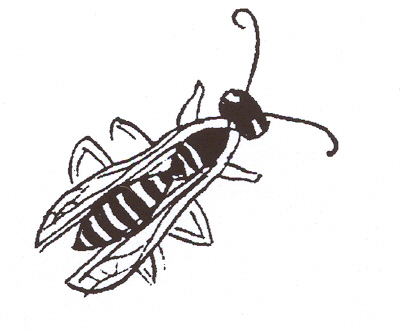
\includegraphics[angle=0,width=24mm,height=36mm]{2.jpg} 
\caption{}
\end{center}
\end{wrapfigure}



\spanenspanenpictureCaptionpictureRightentryletDatadicBody{Kitchen Cooking}
\end{center} \end{adjustwidth}  
\leftmargin 0pt{\markboth{ \headwordentryletDatadicBody అట్లాంటిక్ సమ్దుర్}{ \headwordentryletDatadicBody అట్లాంటిక్ సమ్దుర్}\headwordentryletDatadicBody{అట్వల్}} \spanenpronunciationpronunciationsentryletDatadicBody{[}\spanggofonipaxemicpronunciationpronunciationsentryletDatadicBody{aṭval}\spanenpronunciationpronunciationsentryletDatadicBody{]} \spanteLexSensepublishStemGlossPubLdsensesensesentryletDatadicBody{వంట చేయుట} \spanggoTeluINexampleexamplessensesensesentryletDatadicBody{తిందన్ సాటి రోజి గాటోంగ్ కుస్రింగ్ అట్వల్.} \spantetranslationLdtranslationsexamplessensesensesentryletDatadicBody{తినడానికి రోజు అన్నము కూరలు వంట చేయడం.} \end{hanglist} \end{adjustwidth} 
\begin{adjustwidth}{1pt}{0pt}{2pt}{9pt}
 \begin{hanglist}[12pt] \item 
\leftmargin 0pt{\markboth{ \headwordentryletDatadicBody అట్వల్}{ \headwordentryletDatadicBody అట్వల్}\headwordentryletDatadicBody{అడంతొర్}} \spanenpronunciationpronunciationsentryletDatadicBody{[}\spanggofonipaxemicpronunciationpronunciationsentryletDatadicBody{aḍantor}\spanenpronunciationpronunciationsentryletDatadicBody{]} \spanenspanengrammaticalinfosensesensesentryletDatadicBody{n} \spanenspanensensesensesentryletDatadicBody{crying} \spanteLexSensepublishStemGlossPubLdsensesensesentryletDatadicBody{ఏడ్వడం} \spanggoTeluINexampleexamplessensesensesentryletDatadicBody{కాండిర్ పుట్త బరొబర్ అడంతెర్.} \spantetranslationLdtranslationsexamplessensesensesentryletDatadicBody{పిల్లలు పుట్టినప్పుడు ఏడుస్తారు.} \end{hanglist} \end{adjustwidth} 
\begin{adjustwidth}{1pt}{0pt}{2pt}{9pt}
 \begin{hanglist}[12pt] \item 
\leftmargin 0pt{\markboth{ \headwordentryletDatadicBody అడంతొర్}{ \headwordentryletDatadicBody అడంతొర్}\headwordentryletDatadicBody{అడ్డంఅసి}} \spanenpronunciationpronunciationsentryletDatadicBody{[}\spanggofonipaxemicpronunciationpronunciationsentryletDatadicBody{aḍḍaṁasi}\spanenpronunciationpronunciationsentryletDatadicBody{]} \end{hanglist} \end{adjustwidth} 
\begin{adjustwidth}{1pt}{0pt}{2pt}{9pt}
 \begin{hanglist}[12pt] \item 
\leftmargin 0pt{\markboth{ \headwordentryletDatadicBody అడ్డంఅసి}{ \headwordentryletDatadicBody అడ్డంఅసి}\headwordentryletDatadicBody{అడ్డబుడ్డ}} \spanenpronunciationpronunciationsentryletDatadicBody{[}\spanggofonipaxemicpronunciationpronunciationsentryletDatadicBody{aḍḍabuḍḍa}\spanenpronunciationpronunciationsentryletDatadicBody{]} \spanenspanengrammaticalinfosensesensesentryletDatadicBody{adj} \spanenspanensensesensesentryletDatadicBody{blockage} \spantexitemteLexSensepublishStemGlossPubLdsensesensesentryletDatadicBody{అడ్డదిడ్డమైన} \spanhixitemhiLexSensepublishStemGlossPubLdsensesensesentryletDatadicBody{बाधा देने वाला} \spanggoTeluINexampleexamplessensesensesentryletDatadicBody{కామ్ కీయ్నెకె ఆడ బుడ్డ అయ్వ.} \spantetranslationLdtranslationsexamplessensesensesentryletDatadicBody{పని చేసేటప్పుడు అడ్డదిడ్డముగా రావద్దు.} \end{hanglist} \end{adjustwidth} 
\begin{adjustwidth}{1pt}{0pt}{2pt}{9pt}
 \begin{hanglist}[12pt] \item 
\leftmargin 0pt{\markboth{ \headwordentryletDatadicBody అడ్డబుడ్డ}{ \headwordentryletDatadicBody అడ్డబుడ్డ}\headwordentryletDatadicBody{అడ్డమ్}} \spanenpronunciationpronunciationsentryletDatadicBody{[}\spanggofonipaxemicpronunciationpronunciationsentryletDatadicBody{aḍḍam}\spanenpronunciationpronunciationsentryletDatadicBody{]} \spanenspanengrammaticalinfosensesensesentryletDatadicBody{adv} \spanenspanensensesensesentryletDatadicBody{across.} \spantexitemteLexSensepublishStemGlossPubLdsensesensesentryletDatadicBody{అడ్డముగా} \spanhixitemhiLexSensepublishStemGlossPubLdsensesensesentryletDatadicBody{आडा} \spanggoTeluINexampleexamplessensesensesentryletDatadicBody{పోడ్దున్ అడ్డమ్ టెప్ప ఆత.} \spantetranslationLdtranslationsexamplessensesensesentryletDatadicBody{సూర్యునికి అడ్డముగా మేఘం వచ్చింది.} \end{hanglist} \end{adjustwidth} 
\begin{adjustwidth}{1pt}{0pt}{2pt}{9pt}
 \begin{hanglist}[12pt] \item 
\leftmargin 0pt{\markboth{ \headwordentryletDatadicBody అడ్డమ్}{ \headwordentryletDatadicBody అడ్డమ్}\headwordentryletDatadicBody{అడ్డమ్ ఆ}} \spanenpronunciationpronunciationsentryletDatadicBody{[}\spanggofonipaxemicpronunciationpronunciationsentryletDatadicBody{aḍḍam ā-}\spanenpronunciationpronunciationsentryletDatadicBody{]} \spanenspanengrammaticalinfoentryletDatadicBody{v} \xsensenumbersensesensesentryletDatadicBody{1}\xsensenumberaftersensesensesentryletDatadicBody{) }\spanenspanensensesensesentryletDatadicBody{object} \spantexitemteLexSensepublishStemGlossPubLdsensesensesentryletDatadicBody{అడ్డుకో} \spanhixitemhiLexSensepublishStemGlossPubLdsensesensesentryletDatadicBody{रोक; बीच में पड} \spanggoTeluINexampleexamplessensesensesentryletDatadicBody{బాబల్ బయ్యెన్ పానెకె కాండి అడ్డమ్ ఆతొర్.} \spantetranslationLdtranslationsexamplessensesensesentryletDatadicBody{నాన అమ్మను కొట్టే టప్పుడు కొడుకు అడ్డుకున్నాడు.} \xsensenumbersensesensesentryletDatadicBody{2}\xsensenumberaftersensesensesentryletDatadicBody{) }\spanenspanensensesensesentryletDatadicBody{obstruct} \spantexitemteLexSensepublishStemGlossPubLdsensesensesentryletDatadicBody{అడ్డగించు} \spanhixitemhiLexSensepublishStemGlossPubLdsensesensesentryletDatadicBody{रोक; मना कर} \spanggoTeluINexampleexamplessensesensesentryletDatadicBody{నిమ్మె దర్బర్‌తె అడ్డమ్ అస్సి వడ్క్‌మా.} \spantetranslationLdtranslationsexamplessensesensesentryletDatadicBody{నువ్వు కూర్చోవడం కన్నా అడ్డంగా మాట్లాడకు.} \end{hanglist} \end{adjustwidth} 
\begin{adjustwidth}{1pt}{0pt}{2pt}{9pt}
 \begin{hanglist}[12pt] \item 
\leftmargin 0pt{\markboth{ \headwordentryletDatadicBody అడ్డమ్ ఆ}{ \headwordentryletDatadicBody అడ్డమ్ ఆ}\headwordentryletDatadicBody{అడ్డంవడి}} \spanenpronunciationpronunciationsentryletDatadicBody{[}\spanggofonipaxemicpronunciationpronunciationsentryletDatadicBody{aḍḍanvaḍi}\spanenpronunciationpronunciationsentryletDatadicBody{]} \spanenspanensensesensesentryletDatadicBody{air coming across} \spanteLexSensepublishStemGlossPubLdsensesensesentryletDatadicBody{అడ్డంగా వచ్చే గాలి} \spanggoTeluINexampleexamplessensesensesentryletDatadicBody{నిన్నెతల్ అడ్డంవడి వాసెర్ మంత.} \spantetranslationLdtranslationsexamplessensesensesentryletDatadicBody{నిన్నటి నుండి అడ్డంగా గాలి వస్తుంది.} \end{hanglist} \end{adjustwidth} 
 \end{multicols}\begin{center}
\topskip 18pt{\baselineskip 18pt{\letterletHeaddicBody{న}}}\end{center} 
 \setlength{\columnsep}{12pt} 
\setlength\columnseprule{0.4pt} 
\begin{multicols}{2}{\raggedright} \begin{adjustwidth}{1pt}{0pt}{2pt}{9pt}
 \begin{hanglist}[12pt] \item 
\leftmargin 0pt{\markboth{ \headwordentryletDatadicBody అడ్డంవడి}{ \headwordentryletDatadicBody అడ్డంవడి}\headwordentryletDatadicBody{-న్గ}} \spanenpronunciationpronunciationsentryletDatadicBody{[}\spanggofonipaxemicpronunciationpronunciationsentryletDatadicBody{nga}\spanenpronunciationpronunciationsentryletDatadicBody{]} \end{hanglist} \end{adjustwidth} 
\begin{adjustwidth}{1pt}{0pt}{2pt}{9pt}
 \begin{hanglist}[12pt] \item 
\leftmargin 0pt{\markboth{ \headwordentryletDatadicBody -న్గ}{ \headwordentryletDatadicBody -న్గ}\headwordentryletDatadicBody{-న్గటల్}} \spanenpronunciationpronunciationsentryletDatadicBody{[}\spanggofonipaxemicpronunciationpronunciationsentryletDatadicBody{ngaṭal}\spanenpronunciationpronunciationsentryletDatadicBody{]} \end{hanglist} \end{adjustwidth} 
 \end{multicols}\begin{center}
\topskip 18pt{\baselineskip 18pt{\letterletHeaddicBody{ు}}}\end{center}
 \setlength{\columnsep}{12pt} 
\setlength\columnseprule{0.4pt} 
\begin{multicols}{2}{\raggedright} \begin{adjustwidth}{1pt}{0pt}{2pt}{9pt}
 \begin{hanglist}[12pt] \item 
\leftmargin 0pt{\markboth{ \headwordentryletDatadicBody -న్గటల్}{ \headwordentryletDatadicBody -న్గటల్}\headwordentryletDatadicBody{-ున్‌}} \spanenpronunciationpronunciationsentryletDatadicBody{[}\spanggofonipaxemicpronunciationpronunciationsentryletDatadicBody{un‌}\spanenpronunciationpronunciationsentryletDatadicBody{]} \spanenspanengrammaticalinfosensesensesentryletDatadicBody{ns} \spanenspanensensesensesentryletDatadicBody{ACC} \end{hanglist} \end{adjustwidth} 
\begin{adjustwidth}{1pt}{0pt}{2pt}{9pt}
 \begin{hanglist}[12pt] \item 
\leftmargin 0pt{\markboth{ \headwordentryletDatadicBody -ున్‌}{ \headwordentryletDatadicBody -ున్‌}\headwordentryletDatadicBody{-ుర్}} \spanenpronunciationpronunciationsentryletDatadicBody{[}\spanggofonipaxemicpronunciationpronunciationsentryletDatadicBody{ur}\spanenpronunciationpronunciationsentryletDatadicBody{]} \spanenspanengrammaticalinfosensesensesentryletDatadicBody{vs} \spanenspanensensesensesentryletDatadicBody{3.M.PL.DIST} \end{hanglist} \end{adjustwidth} 
 \end{multicols}\begin{center}
\topskip 18pt{\baselineskip 18pt{\letterletHeaddicBody{ొ}}}
 \label{last_pageొ} 
\end{center}
 \setlength{\columnsep}{12pt} 
\setlength\columnseprule{0.4pt} 
\begin{multicols}{2}{\raggedright} \begin{adjustwidth}{1pt}{0pt}{2pt}{9pt}
 \begin{hanglist}[12pt] \item 
\leftmargin 0pt{\markboth{ \headwordentryletDatadicBody -ుర్}{ \headwordentryletDatadicBody -ుర్}\headwordentryletDatadicBody{-ొర్}} \spanenpronunciationpronunciationsentryletDatadicBody{[}\spanggofonipaxemicpronunciationpronunciationsentryletDatadicBody{or}\spanenpronunciationpronunciationsentryletDatadicBody{]} \spanenspanengrammaticalinfosensesensesentryletDatadicBody{vs} \spanenspanensensesensesentryletDatadicBody{3.M.SG} \end{hanglist} \end{adjustwidth} 
 \end{multicols}
\end{document}
